\section{命名空间}
C++为我们提供了丰富的函数、类和对象,我们只需要若干 \lstinline@#include@ 指令就可以把我们需要的功能收入囊中。这很方便,但也可能导致一些问题。笔者有一次在调尝试调用自己写的 \lstinline@swap@ 函数:
\begin{lstlisting}
void swap(int &a, double &b) {
    int tmp {a};
    a = b;
    b = tmp;
}
int main() {
    int a {3};
    double b {5};
    swap(a, b);
    cout << a << ' ' << b; //预期输出5 3
}
\end{lstlisting}
这段代码的调试结果合乎预期,而当我把 \lstinline@double b{5}@ 改成 \lstinline@int b{5}@ 的时候,却也输出了同样的内容。\par
但是不应该啊,按理说 \lstinline@int@ 类型的 \lstinline@b@ 会转换成 \lstinline@double@ 类型的临时变量,但这个临时变量是右值\footnote{我们将在精讲篇谈左值/右值的问题。},不可能被 \lstinline@swap@ 接收。为什么这个函数仍然正常运行并且给出了``正确''的输出呢?\par
再深入研究之后我才发现,原来程序很本就没有调用我自定义的 \lstinline@swap@ 函数,它调用的是标准库自带的 \lstinline@swap@!
\begin{lstlisting}
template< class T >
void swap( T& a, T& b ) noexcept( /* ... */ );
\end{lstlisting}
也就是从这个时期起,我逐渐改掉了使用 \lstinline@using namespace std@ 和 \lstinline@#include<bits/stdc++.h>@\footnote{\lstinline@bits/stdc++.h@ 是GCC编译器中允许的一个不标准的头文件。使用这个头文件可以让我们一次性包含许多常见头文件。这种用法被普遍认为是``不好的习惯'',详见\href{https://stackoverflow.com/questions/31816095/why-should-i-not-include-bits-stdc-h}{Why should I not \#include <bits/stdc++.h>? - Stack Overflow}。}这两个习惯。\par
几乎所有初学者都会无一例外地认为 \lstinline@using namespace std@ 是很方便的;而通篇累牍的 \lstinline@std::cin@ 和 \lstinline@std::cout@ 则显得十分麻烦。但是当我们的代码量非常大之后,我们难免会起一些与标准库中名字相冲突的变量、函数、枚举、结构和类。举几个例子吧:
\begin{itemize}
    \item \lstinline@list@, \lstinline@map@, \lstinline@array@, \lstinline@queue@, \lstinline@set@, \lstinline@string@, \lstinline@pair@;
    \item \lstinline@copy@, \lstinline@find@, \lstinline@move@, \lstinline@search@, \lstinline@count@, \lstinline@sample@;
    \item \lstinline@next@, \lstinline@begin@, \lstinline@end@, \lstinline@data@, \lstinline@size@;
    \item \lstinline@function@, \lstinline@future@, \lstinline@thread@, \lstinline@yield@;
    \item \ldots\ldots
\end{itemize}
以上这些,有些是类模版,有些是函数模版,或者还有别的。这些名字你可能未必都知道,但是总会有些单词是你熟悉的吧!万一某天你在发愁要起什么名字的时候突然想到了它们——那可能就是问题的根源了。\par
试想,当你在用这些名字定义函数的时候,你是在重载它们;而当你在用这些名字定义类的时候,你会被编译器禁止(因为类不能重载)。被编译器禁止还是更好的选择,因为它在编译期就能帮你检查出错误来;但如果把这些错误留到运行期,那就很难说会发生什么了!\par
解决这个问题的方法很多样。我们可以自己有意识地避开这些名字(一般来说,只要你经验丰富,就不太容易在这个问题上翻车);或者干脆点,不用 \lstinline@using namespace std@ 了\footnote{不过我并不建议读者彻底杜绝 \lstinline@using namespace std@ 的使用。这种语法并不像 \lstinline@bits/stdc++.h@ 库或 \lstinline@goto@ 语句那样饱受诟病,仍然是许多程序员图省事的最佳选择。}。那么究竟什么是 \lstinline@namespace@,我们为什么要用它,又怎么用它呢?本节就来讲解这些问题。\par
\subsection*{什么是命名空间?}
想象一下Windows电脑的文件资源管理器——就以D盘为例吧。我们可以直接把文件存放在D盘的主目录下,不过我们很少这么做;我们绝大多数时候是在D盘中建立一些文件夹,甚至是文件夹套文件夹,然后把具体的文件存放到这些文件夹中。简化起见,我们只在D盘中用两个文件夹。这两个文件夹中各有一份名叫\texttt{Test.txt}的文本文档\footnote{它们二者之间不是快捷方式的关系,是真正意义上独立的文件。否则这个讨论就没什么意义了。}。它们虽然同名,但它们不冲突,因为它们在不同的文件夹下。修改其中一个\texttt{Test.txt}中的内容也不会对另一个\texttt{Test.txt}造成什么影响。\par
那么我们是不是可以这样认为:这两个文件虽然重名,但它们存在于不同的空间中,所以不会有什么冲突。如果我们想访问这两个文件,我们也肯定会通过不同路径来找。这样,一切可能的冲突都解决了。\par
\begin{figure}[htbp]
    \centering
    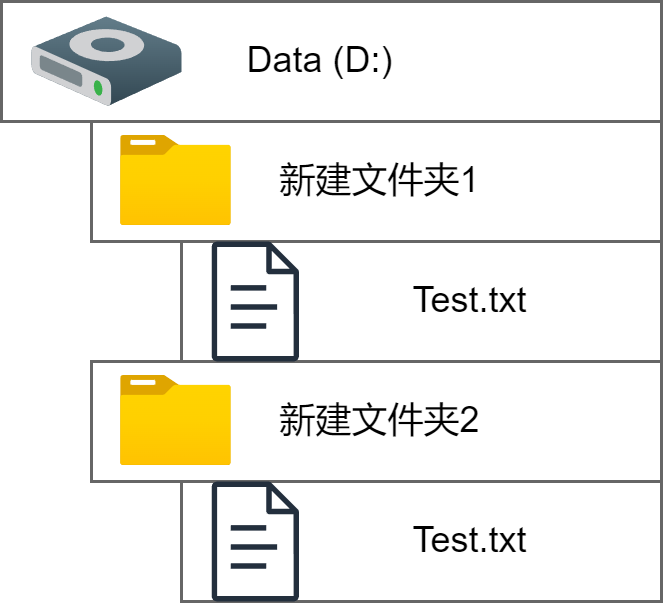
\includegraphics[width=0.5\textwidth]{../images/generalized_parts/07_file_explorer_and_namespaces_300.png}
    \caption{Windows文件资源管理器中的重名文件}
\end{figure}
命名空间也是这样的道理。在不同的命名空间中,我们可以按我们的需要来给变量、函数和类起名字,而不必担心与其它命名空间中的什么东西重名。\par
不过,实际上的命名空间还是与Windows资源管理器的结构不同的。接下来我们讲解一些有关命名空间的最基本规则。\par
\subsection*{命名空间的层级}
